% Assignment 2 research report. Build from assignment2/report/ with:
%   tectonic -X compile main.tex
% Tables and figures are read from ../analysis (generated by analysis/analyze.py).
\documentclass[11pt,a4paper]{article}

\usepackage[T1]{fontenc}
\usepackage{lmodern}
\usepackage{microtype}
\usepackage[margin=2.4cm]{geometry}
\usepackage{amsmath}
\usepackage{booktabs}
\usepackage{array}
\usepackage{graphicx}
\usepackage{xcolor}
\usepackage{listings}
\usepackage[font=small,labelfont=bf]{caption}
\usepackage{subcaption}
\usepackage{enumitem}
\usepackage[hidelinks]{hyperref}
\usepackage{url}

\graphicspath{{../analysis/figures/}}
\newcommand{\tabledir}{../analysis/tables}
\newcommand{\repourl}{\url{https://github.com/Xami650/Individual-Assignments-Big-Data-ULPGC}}
\newcommand{\session}{\texttt{20261029-104152}}

\lstset{
  basicstyle=\ttfamily\footnotesize,
  columns=fullflexible,
  keepspaces=true,
  frame=single,
  framesep=3pt,
  rulecolor=\color{black!30},
  aboveskip=4pt,
  belowskip=2pt,
  showstringspaces=false,
}

\setlist{itemsep=2pt,topsep=4pt}

\title{\textbf{Assignment 2: Optimised Dense and Sparse Matrix Multiplication}\\[4pt]
\large Loop Reordering, Cache Blocking and a CSR Product Against the Basic Triple Loop in Java}
\author{Máximo Prosperi Reynoso\\[2pt]
\small BIG DATA, GCID, ULPGC\\
\small Individual Assignment 2, 2026--2027\\[2pt]
\small \repourl}
\date{30 October 2026}

\begin{document}
\maketitle

\begin{abstract}
\noindent
This study asks how two optimisations change sequential dense matrix
multiplication in Java, and when a sparse representation pays off. Part~A
compares the validated i-j-k baseline of Assignment~1 with loop reordering
(i-k-j) and cache blocking, for $n=64$ to 4096. Part~B compares a CSR product
(Gustavson's algorithm) with the blocked dense method on the same matrices: at
$n=2048$ for densities from 0.1 to 50\%, with uniformly scattered and with
banded nonzeros, and at 1\% density for $n$ up to 32768. Every method gave
bitwise-identical results. Reordering made the kernel 3.1 to 10 times faster.
It cut the instructions per multiply-add from about 12 to 3 to 4.6, a count
consistent with vectorised code, and it removed the stall cycles of the
baseline. Blocking added nothing up to $n=2048$, but it was 1.2 to 1.6 times
faster than i-k-j at $n=3072$ and 4096, where the i-k-j stream through $B$
started to stall. The CSR product was 7 to 26\,000 times faster than blocked at
densities up to 10\%, and 2.6 times slower at 50\%. At equal density and equal
work, banded inputs produced up to 5.3 times fewer output nonzeros and ran up to
2.2 times faster than uniform ones, so density alone did not determine the
cost. Converting dense inputs to CSR cost more than the product at 0.1\%
density. At 1\% density the dense method exceeded the 120\,s budget at
$n=16384$, and the sparse one ran out of the 8\,GiB heap at $n=32768$, where
its output fills in. The conclusions hold for the tested methods, inputs and
machine only.
\end{abstract}

% ===========================================================================
\section{Introduction and objective}

Assignment~1 measured the basic triple-loop matrix multiplication in Python, Java
and C. Its runtime grew faster than $n^3$, and the process counters located the
cause in the memory system: the instructions per inner iteration stayed constant
while the cycles per iteration rose with $n$. The inner loop of the i-j-k order
walks a column of $B$, one row apart in memory at every step. That study left the
remedies, ``loop orders that walk $B$ along its rows'', to this assignment. This
study keeps one language, Java, and one baseline, the validated Java kernel of
Assignment~1, and asks two questions.

\paragraph{Part A: dense optimisation.} \emph{How do loop reordering (i-k-j) and
cache blocking change the runtime and memory of sequential dense matrix
multiplication, relative to the basic i-j-k baseline, as the size $n$ grows?}
The factor is the method and $n$, with the tile size as a secondary factor. The
outcomes are the time per multiplication, the peak memory of the process and its
instruction and cycle counts.

\paragraph{Part B: sparse matrices.} \emph{Under which tested densities and
nonzero structures does a sparse product in compressed sparse row (CSR) format
run faster or use less memory than the optimised dense method on the same
logical matrices, and which costs reduce its advantage?} The factors are the
density, the structure of the nonzeros and $n$. Throughout this report, the
\emph{density} is the percentage of nonzero entries of a matrix and the
\emph{sparsity} is the percentage of zero entries, so a density of 1\% is a
sparsity of 99\%.

\paragraph{Hypotheses.} The hypotheses below were fixed in the protocol file
(\texttt{config/bench.json}) before the reported session. They are predictions,
and Section~\ref{sec:discussion} tests them against the results.
\begin{itemize}
  \item[HA1] ikj is several times faster than basic from $n=256$ upward, and the
  gap grows with $n$: its inner loop reads $B$ and $C$ along rows and its
  iterations are independent, so the JIT compiler can vectorise it.
  \item[HA2] blocked is no faster than ikj while ikj's row-wise stream through
  $B$ is served quickly enough, and becomes faster only at the largest sizes.
  Tiles sized for the L1 cache gain nothing over larger, L2-sized tiles.
  \item[HA3] All methods, the sparse one included, produce bitwise-identical
  results, because each adds the same products to $C_{ij}$ in increasing $k$.
  \item[HA4] The optimisations change runtime but not memory.
  \item[HB1] The sparse kernel's time follows its number of multiply-adds
  (expected $n^3d^2$ at density $d$) plus the size of its output; dense time does
  not depend on the density.
  \item[HB2] At equal density and equal multiply-add count, banded inputs give
  far fewer output nonzeros than uniformly scattered ones, so density alone does
  not determine performance.
  \item[HB3] At $n=2048$, the sparse product is faster than blocked at low
  densities and loses that advantage between 5\% and 50\% density for uniform
  inputs; the break-even density is higher for banded inputs.
  \item[HB4] CSR storage is smaller than dense storage below about 67\% density,
  but for uniform inputs of 5\% density and more the product fills in so much
  that its CSR form is larger than its dense form.
  \item[HB5] When the inputs arrive dense, converting them to CSR outweighs the
  sparse kernel at low densities.
  \item[HB6] At a fixed density, the dense method is limited by time and the
  sparse one by the memory of its output.
\end{itemize}

% ===========================================================================
\section{Background and references}

\paragraph{Loop order.} With row-major storage, the i-j-k loop reads row $i$ of
$A$ with unit stride but column $j$ of $B$ with a stride of one full row, so
consecutive accesses to $B$ fall in different cache lines and, for large $n$,
in different pages. Exchanging the two inner loops gives the i-k-j order, in
which the innermost loop adds a multiple of row $k$ of $B$ to row $i$ of $C$;
both are read sequentially~\cite{bryant2016,drepper2007}. The i-k-j inner loop
has a second property: its iterations are independent of each other, whereas
the i-j-k inner loop chains every addition through one scalar. Independent
iterations can be executed several at a time with SIMD instructions. HotSpot's
C2 compiler does this automatically for simple loops with its SuperWord pass,
which follows the superword-level-parallelism method of Larsen and
Amarasinghe~\cite{larsen2000}. On the Apple M4 the vectors are 128-bit NEON
registers, which hold two doubles.

\paragraph{Cache blocking.} Blocking (tiling) splits the loops into tiles so
that a tile of each matrix is reused many times while it stays in
cache~\cite{lam1991}. High-performance libraries block for every level of the
memory hierarchy and add register-level micro-kernels~\cite{goto2008}. This
study implements only the textbook form: three tile loops around the i-k-j
loop.

\paragraph{Order of operations.} Floating-point addition is not associative, so
different summation orders give slightly different results~\cite{higham2002}.
In every method of this study, each $C_{ij}$ receives the products
$A_{ik}B_{kj}$ in increasing $k$, starting from $0.0$. The sparse product skips
products that are exactly zero, and adding $\pm0$ to a sum does not change it.
Java forbids contracting $a\cdot b+c$ into a fused multiply-add~\cite{jep306}.
All methods therefore perform the same rounded operations in the same order
for every entry, and they should agree bit for bit (HA3).

\paragraph{Sparse storage and multiplication.} The CSR format stores the
nonzeros of a matrix row by row: an array of values, an array with the column
index of each value, and an array of $n+1$ row pointers that marks where each
row starts~\cite{saad2003}. With 8-byte values and 4-byte indices, a CSR matrix
takes $12\,\mathrm{nnz}+4(n+1)$ bytes against $8n^2$ for the dense form, so it is
smaller below a density of about $2/3$. Gustavson's algorithm computes $C=AB$ row
by row: for each nonzero $A_{ik}$, it adds $A_{ik}$ times row $k$ of $B$ into a
dense accumulator for row $i$ of $C$~\cite{gustavson1978}. Its work is
proportional to the number of multiply-adds, $\sum_{(i,k)\in A}\mathrm{nnz}(B_{k,:})$,
plus the size of the output, and not to $n^3$~\cite{gilbert1992,davis2006}.
For two matrices whose $d n^2$ nonzeros are placed independently and uniformly
at random, the expected number of multiply-adds is $n^3d^2$, and an entry of $C$
is structurally nonzero with probability $1-(1-d^2)^n$. At $n=2048$ this is
about 18\% for $d=1\%$ and over 99\% for $d=5\%$: the product can be far denser
than its factors.

\paragraph{JIT warm-up.} A Java method that runs for seconds per call is first
executed by the interpreter and then by code that the JIT compiles while the
loop is running (on-stack replacement, OSR). Its first calls can therefore run
code of a different quality from the steady state, which is why benchmarks
discard warm-up iterations~\cite{georges2007}. Section~\ref{sec:protocol}
describes a case where this mattered.

% ===========================================================================
\section{Methodology}
\label{sec:method}

\subsection{Implementations}

All code is in \texttt{src/main/java/org/ulpgc/bd/matmul/} and was written for
this study, except the baseline, which is copied unchanged from
Assignment~1. No library is used in any measured method. Every method computes
in IEEE-754 double precision on one thread. The dense methods share the storage
of Assignment~1, \texttt{double[][]} (an array of row arrays), so that they
differ only in their loops (Fig.~\ref{fig:kernels}).
\begin{itemize}
  \item \textbf{basic} (baseline, \texttt{DenseMatMul.basic}): the i-j-k loop with
  a scalar accumulator from Assignment~1 (tag \texttt{assignment1-v1.0}), where it
  was validated against NumPy and the C and Python versions.
  \item \textbf{ikj} (loop reordering, \texttt{DenseMatMul.ikj}): the i-k-j order.
  Row $i$ of $C$ is cleared, then each $A_{ik}$ times row $k$ of $B$ is added to it.
  \item \textbf{blocked} (cache blocking, \texttt{DenseMatMul.blocked}): the ikj
  loop split into tiles of $b$ indices in each dimension, with tile loops in the
  order $ii$, $kk$, $jj$. The tile loop over $k$ is ascending for every $(i,j)$,
  which keeps the order of the additions. The tile size of the main experiments
  is $b=512$: three $512\times512$ tiles take 6\,MiB and fit in the 16\,MiB L2
  cache of the performance cores. Section~\ref{sec:protocol} explains how this
  size was chosen, and experiment A\_block re-measures the alternatives.
  \item \textbf{csr} (sparse product, \texttt{CsrMatrix.multiply}): canonical CSR
  (column indices increasing within each row; \texttt{int} indices, so at most
  $2^{31}-1$ nonzeros) and Gustavson's algorithm in two passes. A symbolic pass
  marks, for each row $i$, the columns reached through the nonzeros of row $i$ of
  $A$, which gives the exact size of $C$; $C$ is then allocated. A numeric pass
  accumulates row $i$ in a dense array of length $n$ and writes the touched
  columns in increasing order: by sorting them, or by scanning the marker array
  when the row holds more than $n/16$ entries. Stored entries are structural
  nonzeros; one whose products cancel to $0.0$ stays stored.
  \item \textbf{to\_csr} and \textbf{to\_dense} (conversions,
  \texttt{CsrMatrix.fromDense} and \texttt{toDense}): dense to CSR for both
  inputs, and the CSR product back to a dense matrix.
\end{itemize}

\begin{figure}[t]
\centering
\begin{subfigure}[t]{0.48\linewidth}
\begin{lstlisting}[language=Java]
// basic (Assignment 1)
for (int i = 0; i < n; i++)
  for (int j = 0; j < n; j++) {
    double s = 0.0;
    for (int k = 0; k < n; k++)
      s += a[i][k] * b[k][j];
    c[i][j] = s;
  }
\end{lstlisting}
\end{subfigure}\hfill
\begin{subfigure}[t]{0.48\linewidth}
\begin{lstlisting}[language=Java]
// ikj
for (int i = 0; i < n; i++) {
  double[] ai = a[i], ci = c[i];
  Arrays.fill(ci, 0.0);
  for (int k = 0; k < n; k++) {
    double aik = ai[k]; double[] bk = b[k];
    for (int j = 0; j < n; j++)
      ci[j] += aik * bk[j];
  }
}
\end{lstlisting}
\end{subfigure}

\medskip
\begin{subfigure}[t]{0.48\linewidth}
\begin{lstlisting}[language=Java]
// blocked (C cleared first)
for (ii = 0; ii < n; ii += bs)
 for (kk = 0; kk < n; kk += bs)
  for (jj = 0; jj < n; jj += bs)
   for (i = ii; i < min(ii+bs, n); i++)
    for (k = kk; k < min(kk+bs, n); k++)
     for (j = jj; j < min(jj+bs, n); j++)
      c[i][j] += a[i][k] * b[k][j];
\end{lstlisting}
\end{subfigure}\hfill
\begin{subfigure}[t]{0.48\linewidth}
\begin{lstlisting}[language=Java]
// csr, numeric pass for row i
for (p in row i of A) {
  k = A.col[p]; aik = A.val[p];
  for (q in row k of B) {
    j = B.col[q];
    if (marker[j] != i) { // new entry
      marker[j] = i; cols[len++] = j;
      acc[j] = 0.0; }
    acc[j] += aik * B.val[q];
  }
} // then order cols, copy acc to C
\end{lstlisting}
\end{subfigure}
\caption{The measured kernels (blocked and csr abbreviated; the code hoists the
row references as in ikj). Every method adds the products of each $C_{ij}$ in
increasing $k$.}
\label{fig:kernels}
\end{figure}

\subsection{Inputs}

\paragraph{Dense inputs (Part A).} The dense inputs are those of
Assignment~1, generated by the same unchanged code: for each $n$, $A$ and then
$B$ are drawn uniformly on $[-1,1)$ from NumPy's PCG64
generator~\cite{harris2020} seeded with \texttt{SeedSequence([2026, n])}, and
stored as raw little-endian float64. For the 14 sizes the two studies share,
the files are byte-identical to Assignment~1's (same SHA-256). Every entry is
nonzero.

\paragraph{Sparse inputs (Part B).} Each sparse matrix has its own PCG64
generator, whose seed sequence holds five integers: 2026, $n$, the structure
(0 or 1), the density in parts per million, and the matrix (0 for $A$, 1 for
$B$). A matrix of density $d$ holds exactly
$\mathrm{round}(d n^2)$ nonzeros at distinct positions drawn without
replacement, followed by their values, drawn uniformly on $[-1,1)$ with exact
zeros redrawn. Two structures give the same nonzero count and the same expected
number of nonzeros per row:
\begin{itemize}
  \item \textbf{uniform}: every position of the matrix is equally likely;
  \item \textbf{banded}: only positions with $|i-j|\le w$, $w=\lceil dn\rceil$,
  are possible, and they are equally likely, so the band is about half full.
\end{itemize}
Both give the same expected multiply-add count, $n^3d^2$, but for banded inputs
$C$ lies within the band $|i-j|\le 2w$, so it has at most about $4dn^2$ nonzeros.
The files store CSR directly (header with $n$ and nnz, then the three arrays).
The SHA-256 digest of every input file is tracked in
\texttt{data/checksums.sha256}.

\subsection{Experiments}

Table~\ref{tab:experiments} lists the four experiments of the reported session.
In Part~B, every method reads the same CSR files. The dense method expands them
to \texttt{double[][]} before the timed region, so the sparse and dense methods
multiply the same logical matrices.

\begin{table}[t]
\centering
\caption{Experiments of the reported session (99 configurations).}
\label{tab:experiments}
\small
\begin{tabular}{@{}l>{\raggedright\arraybackslash}p{0.27\linewidth}>{\raggedright\arraybackslash}p{0.5\linewidth}@{}}
\toprule
Experiment & Methods & Inputs \\
\midrule
A\_dense & basic, ikj, blocked ($b=512$) & dense; $n=64$, 128, 256, 384, 512, 768, 1024, 1536, 2048, 3072, 4096 \\
A\_block & blocked, $b=32$, 64, 128, 256, 512 & dense; $n=2048$, 4096 \\
B\_density & csr, blocked, to\_csr, to\_dense & $n=2048$; density 0.1, 0.5, 1, 5, 10 and 50\% (sparsity 99.9 to 50\%); uniform and banded \\
B\_size & csr, blocked & uniform, density 1\%; $n=1024$, 2048, 4096, 8192, 16384, 32768 \\
\bottomrule
\end{tabular}
\end{table}

\subsection{Execution environment}

Table~\ref{tab:env} lists the machine and the software. These settings were
fixed for every run.

\begin{table}[t]
\centering
\caption{Execution environment and fixed settings of the reported session
(\session, recorded in \texttt{env.txt} before and after the session).}
\label{tab:env}
\small
\begin{tabular}{@{}lp{0.72\linewidth}@{}}
\toprule
Machine & MacBook Air (Mac16,13), fanless; 24\,GiB RAM; AC power, Low Power Mode off \\
CPU & Apple M4: 4 performance cores (L1d 128\,KiB each, 16\,MiB L2 shared) and
6 efficiency cores (L1d 64\,KiB, 4\,MiB L2); 10 logical processors; 128\,B cache
line; 16\,KiB pages \\
OS & macOS 26.6.2 (build 25G83), Darwin 25.6.0 \\
Java & OpenJDK 25.0.2 (HotSpot 64-bit Server VM), Maven 3.9.12;
\texttt{java -Xmx8g}; defaults otherwise: G1 collector (4\,MiB regions), tiered
compilation with 4 compiler threads, 9 parallel and 2 concurrent GC threads,
SuperWord vectorisation on, 16-byte maximum vector size \\
Python & CPython 3.13.9 (Anaconda build) with NumPy 2.3.5, SciPy 1.16.3,
pandas 2.3.3 and matplotlib 3.10.6, only for inputs, checks and analysis \\
Threads & every measured method runs on one thread; the JVM adds its own JIT
and GC threads \\
Source & commit \texttt{acf4520} (all code of the session committed) \\
Conditions & session of 42.2\,min; no thermal or performance warning recorded
before or after; load average 5.1 at the start and 2.0 at the end, with
desktop applications open \\
\bottomrule
\end{tabular}
\end{table}

\subsection{Correctness checks}
\label{sec:correctness}

The Java code has 45 JUnit~5 tests. They cover hand-computed $2\times2$ and
$3\times3$ products, identity and zero matrices, the overwriting of a reused
output buffer, an exact BigDecimal reference, sizes that are not multiples of
the tile size, and the bitwise equality of ikj and blocked (with tile sizes 1 to
512) to basic. For the sparse code, they cover the conversions, empty rows, a
structural nonzero that cancels to $0.0$, the nonzero and multiply-add counts
against a brute-force count, and bitwise equality to the dense baseline for
densities from 1\% to 100\%. Further tests cover the file formats and the
driver's output contract.

Before benchmarking, \texttt{scripts/verify.py} ran every method through its
normal command line. The dense cases follow Assignment~1:
$n\in\{1,2,3,10,64,100,256\}$, with random inputs (reference
\texttt{numpy.matmul}), $AI$ (exact answer $A$) and $A\cdot0$ (exact answer $0$),
for basic, ikj and blocked with tile sizes 7, 64 and 512. The sparse cases cover
both structures, $n\in\{1,10,100,256\}$ and densities 0, 1, 10, 50 and 100\%,
for csr, to\_dense and the three dense methods. Their reference is the SciPy CSR
product~\cite{virtanen2020}. The structural nonzero count of $C$ comes from the
product of the 0/1 patterns, and csr must store exactly that many entries.
SciPy and NumPy serve only as checks and are not compared methods. A result
passes if $|C_{ij}-R_{ij}|\le 2\gamma_n(|A||B|)_{ij}$ for every entry, with
$\gamma_n=nu/(1-nu)$ and $u=2^{-53}$. This is the tolerance of Assignment~1. It
bounds the difference between two results computed in any summation
order~\cite{higham2002}, and the $|A||B|$ scaling also covers entries that cancel
to zero. During the benchmark, every sample prints a checksum of its result,
which consumes the result and is compared across methods.

\subsection{Measurement protocol}
\label{sec:protocol}

The protocol is that of Assignment~1, with one addition, the JIT pre-warm.

\paragraph{Timer boundary.} Only the operation of the method is timed, with
\texttt{System.nanoTime()}. For the dense methods this is the kernel call,
including the clearing of $C$ that ikj and blocked perform. For csr it is the
whole \texttt{CsrMatrix.multiply} call: both passes, the allocation of $C$ and
the ordering of its columns. The conversions are timed separately as their own
methods (to\_csr converts $A$ and $B$; to\_dense converts $C$). The csr kernel
time therefore \emph{excludes} conversion, and the conversion costs are
\emph{measured separately} and added where a comparison needs them. Loading the
inputs, converting them to the method's representation and starting the JVM are
outside the timed region. A method that allocates its result drops the previous
one before each call.

\paragraph{Pre-warm, warm-up and samples.} Each configuration runs in one fresh
JVM. Before any sample, the driver runs the method for 1\,s on small random
inputs ($n=\min(N,256)$, densities 2\% and 50\%), so that the JIT compiles it
with a complete profile. This step is new. In a pilot run without it, ikj at
$n=2048$ took 3.3\,s per multiplication in every sample, against 1.24\,s with
it. \texttt{-XX:+PrintCompilation} showed why: the first call ran OSR-compiled
code, the fully compiled method was deoptimised (``uncommon trap'') when its
loops exited for the first time, and the later calls ran C1-compiled code.
Without the pre-warm, the comparison would have measured the JIT's state rather
than the method. Warm-up then continues until at least 1\,s of warm-up work and
at least one sample have run. Each sample times $k$ back-to-back operations; the
first warm-up uses $k=1$, and every later sample uses
$k=\max(1,\lceil 0.1\,\text{s}/t\rceil)$, where $t$ is the time per operation of
the latest warm-up. Five measured samples follow. The summaries report the
median and the interquartile range (IQR) of the time per operation over the
five measured samples. Warm-up samples are kept in the raw data and excluded
from every summary.

\paragraph{Budgets and run order.} The budgets were declared before the session.
Each process had 60\,s to load and convert its inputs and pre-warm, and then at
most 120\,s for every sample. The heap was limited to 8\,GiB
(\texttt{-Xmx8g}, the same flags for every run). A process that missed a
deadline was killed and recorded as a timeout. One whose JVM ran out of heap
exited with a distinct status, recorded as a memory failure. In both cases the
larger sizes of the same series were skipped. The session budget was 90\,min. The
experiments ran in the order of Table~\ref{tab:experiments}, with $n$ ascending,
and with a 2\,s pause between processes.

\paragraph{Pilot.} Single-run pilots, not part of the reported data, set the
largest sizes, the time budget and the tile size. Tiles of $b=16$ to 512 were
timed once at $n=2048$ and 4096; $b=512$ was the fastest at $n=4096$. The pilot
is the source of the tile size declared in the protocol, and experiment A\_block
repeats the comparison under the full protocol.

\paragraph{Memory metrics and counters.} Every process ran under
\texttt{/usr/bin/time -l}. It reports the peak resident set size (RSS) of the
whole process, as in Assignment~1, and the peak memory footprint. Unlike RSS,
the footprint also counts pages that macOS has compressed, which a pilot showed
to matter above about 8\,GB. Both measure the whole process: JVM, inputs,
conversions and garbage not yet collected. The second metric is the element
storage of each representation, computed from $n$ and the nonzero counts:
$8n^2$ bytes per dense matrix and $12\,\mathrm{nnz}+4(n+1)$ per CSR matrix. The
same tool reports the instructions retired and the cycles of the process. For
the dense methods, these are divided by every multiply-add the process ran
(pre-warm, warm-up and measured samples).

% ===========================================================================
\section{Results}
\label{sec:results}

The session ran 99 configurations in 42.2\,min, of which 95 completed. Two exceeded the
time budget: basic at $n=4096$ and blocked at $n=16384$ (1\% density). One ran
out of heap: csr at $n=32768$. One was skipped after a failure: blocked at
$n=32768$. Every completed configuration has five measured samples. The largest
relative IQR is 3.9\%, and the median is 0.5\%.

\subsection{Correctness}

All 45 unit tests passed. \texttt{verify.py} checked 305 (case, method) results:
all were within the tolerance (largest error 0.13 of the bound), every method
was bitwise identical to every other on each case, and csr stored exactly the
structural nonzero count of $C$ in all 40 sparse cases. In the benchmark session,
the checksums of every method that computes $C$ agreed exactly on each of the 27
inputs (83 configurations).

\subsection{Part A: dense methods}

Table~\ref{tab:dense} and Fig.~\ref{fig:dense} give the time per multiplication.
ikj was 3.1 times faster than basic at $n=64$, and the ratio grew with $n$ to
about 10 at $n=2048$ and 3072. Up to $n=2048$, blocked stayed within 0.88 to 1.03
times ikj's speed. It was slower at $n=768$, 1024 and 2048 and level elsewhere. At
$n=3072$ and 4096 it was faster, by factors of 1.57 and 1.21. The baseline took
67.9\,s at $n=3072$ and exceeded the 120\,s budget at $n=4096$. The largest size
within budget is therefore 3072 for basic and at least 4096, the largest size
attempted, for ikj and blocked. Fitted between $n=256$ and the largest completed
size, the log-log slope of the time is 3.59 for basic, 3.18 for ikj and 3.08 for
blocked.

\begin{table}[t]
\centering
\caption{Part A: median time per multiplication in ms (relative IQR), five
measured samples per cell, and time ratios between the methods (above 1: the
second method is faster).}
\label{tab:dense}
\small
\input{\tabledir/tab_dense_time.tex}
\end{table}

\begin{figure}[t]
\centering
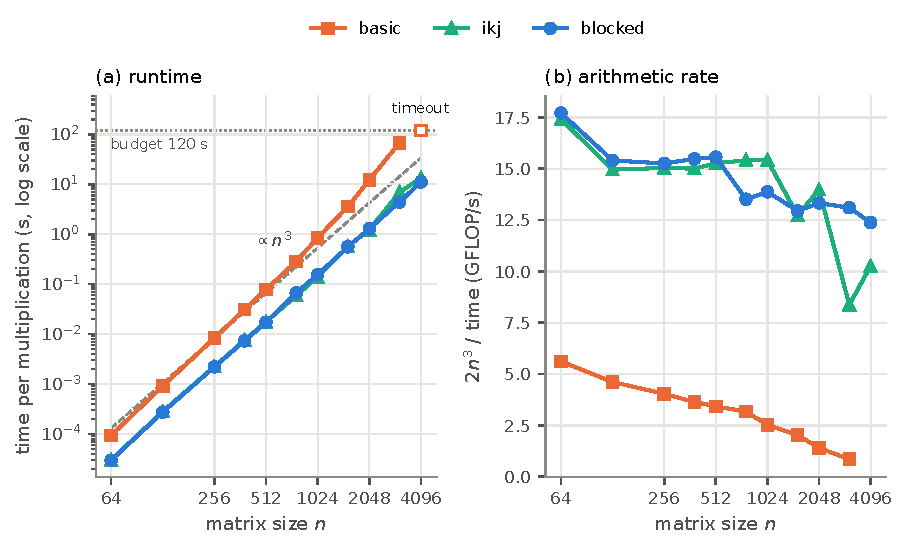
\includegraphics[width=\linewidth]{fig_dense.pdf}
\caption{Part A. (a) Median time per multiplication (log-log), with IQR bars
(smaller than the markers) and an $n^3$ guide; the hollow marker is basic's
timeout at $n=4096$. (b) Arithmetic rate, $2n^3$ divided by the median time.}
\label{fig:dense}
\end{figure}

Table~\ref{tab:counters} normalises the process counters by every multiply-add
the process ran. Basic retired 11.5 to 12.2 instructions per multiply-add at
every size, as in Assignment~1, while its cycles per multiply-add rose from 1.5
to 9.3. ikj retired 2.9 to 4.6 instructions per multiply-add, and blocked 3.4
to 4.5. Up to $n=2048$, both needed 0.48 to 0.63 cycles per multiply-add, about
13 to 18\,GFLOP/s. At $n=3072$ and 4096 ikj rose to 0.96 and 0.79 cycles per
multiply-add, while blocked stayed at 0.62. ikj was therefore slower per
multiply-add at $n=3072$ than at 4096. For the dense methods, the timed
operations accounted for 58 to 100\% of the process's user CPU time. The lower
values belong to small and medium $n$, where the 1\,s pre-warm is a large part
of the process.

\begin{table}[t]
\centering
\caption{Part A: process counters per multiply-add (pre-warm, warm-up and
measured samples) and arithmetic rate of the median.}
\label{tab:counters}
\small
\input{\tabledir/tab_dense_counters.tex}
\end{table}

The peak RSS of the three dense methods differed by at most 1.1\,MiB at every
size (Table~\ref{tab:densemem}). It grew from a 52\,MiB baseline to 393\,MiB at
$n=3072$ and 544\,MiB at $n=4096$, 28 to 58\% more than the $24n^2$ bytes of the
three matrices above the baseline.

\begin{table}[t]
\centering
\caption{Part A: peak RSS in MiB, and the element storage of three dense
matrices.}
\label{tab:densemem}
\small
\input{\tabledir/tab_dense_memory.tex}
\end{table}

Table~\ref{tab:block} and Fig.~\ref{fig:block} show the tile sizes. At
$n=2048$, every tile size was slower than ikj: blocked took 1.05 ($b=512$) to
1.47 ($b=32$) times as long. At $n=4096$, the gain over ikj grew with the tile
size, from a 7\% loss at $b=32$ to a 1.21-fold gain at $b=512$.

\begin{table}[t]
\centering
\caption{Part A: blocked with tile sizes $b=32$ to 512, median time in s
(relative IQR), and the time of ikj divided by that of blocked.}
\label{tab:block}
\small
\input{\tabledir/tab_block.tex}
\end{table}

\begin{figure}[t]
\centering
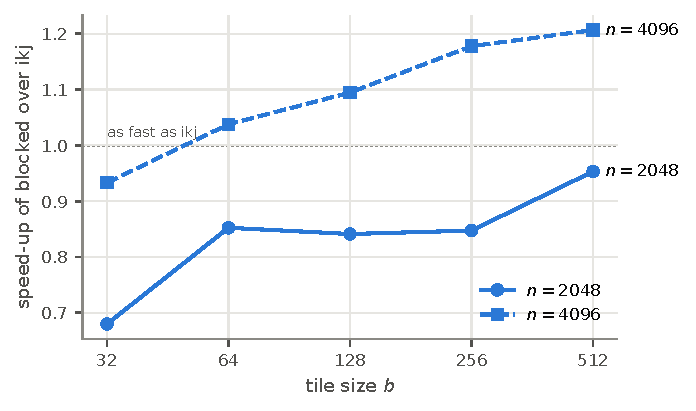
\includegraphics[width=0.62\linewidth]{fig_block.pdf}
\caption{Part A: speed-up of blocked over ikj against the tile size (medians).}
\label{fig:block}
\end{figure}

\subsection{Part B: density and structure at $n=2048$}

Table~\ref{tab:density} and Fig.~\ref{fig:density} compare csr with blocked on
the same matrices. The dense method's time did not depend on the input: it
stayed between 1\,301 and 1\,331\,ms for every density and both structures. csr
took 0.06\,ms at 0.1\% density and 3.4\,s at 50\%. It was faster than blocked at
every density up to 10\%: 22\,485 to 7.0 times for uniform inputs and 25\,672 to
8.2 times for banded ones. At 50\% it was 2.6 and 2.7 times slower. The tested
densities do not locate the break-even more precisely than between 10\% and
50\%. A log-linear interpolation of the speed-up between those two points places
it near 30\% for both structures. This is an estimate, not a measurement.

\begin{table}[t]
\centering
\caption{Part B at $n=2048$: nonzero counts (nnz($B$) equals nnz($A$); nnz($C$)
in thousands, with the density of $C$), multiply-adds of the sparse product in
millions, median times in ms (relative IQR at most 3.2\%), and speed-up of csr
over blocked for the kernel alone and including both conversions (to\_csr +
csr + to\_dense).}
\label{tab:density}
\footnotesize
\setlength{\tabcolsep}{3.5pt}
\resizebox{\linewidth}{!}{\input{\tabledir/tab_density.tex}}
\end{table}

\begin{figure}[t]
\centering
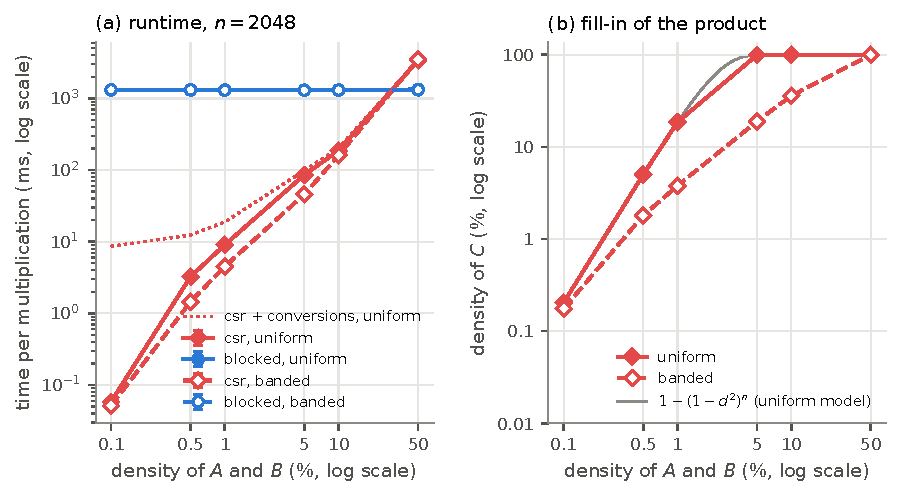
\includegraphics[width=\linewidth]{fig_density.pdf}
\caption{Part B at $n=2048$. (a) Median time per multiplication against the input
density; solid lines and filled markers are uniform inputs, dashed lines and
hollow markers banded ones; the blocked lines for the two structures coincide.
The dotted line adds both conversions to csr (uniform). (b) Density of the
product $C$, with the expected value for uniform inputs.}
\label{fig:density}
\end{figure}

At equal density, the two structures had the same nonzero count and nearly the
same number of multiply-adds (within 1.6\% up to 10\%, 3.7\% at 50\%), but very
different products. For uniform inputs, $C$ followed the model
$1-(1-d^2)^n$ closely: 5.0\% dense at 0.5\%, 18.5\% at 1\% and 99.4\% at 5\%. For
banded inputs, $C$ had 2.8 to 5.3 times fewer nonzeros between 0.5 and 10\%
density. csr ran 2.2, 2.0, 1.9 and 1.2 times faster on banded than on uniform
inputs at 0.5, 1, 5 and 10\%. At 50\%, both products were full and the times
were equal within 3\%. The time per multiply-add of csr fell with the density,
from 15\,ns (uniform, 0.5\%) and 6.8\,ns (banded) to 1.6\,ns at 50\%.

Converting both inputs to CSR took 7.3 to 7.9\,ms up to 1\% density and 36\,ms
at 50\% (uniform). That is 127 times the csr kernel at 0.1\%, about as much as the
kernel at 1\% (uniform), and 1 to 21\% of it from 5\% upward. Converting
the product back to dense took 1.1 to 2.7\,ms. With both conversions included,
the speed-up over blocked fell from 22\,485 to 152 at 0.1\% and from 145 to 69 at
1\% (uniform). From 5\% upward it fell by 1 to 20\%.

Table~\ref{tab:densitymem} gives the memory. The CSR inputs took 0.1 to 48\,MiB,
against 64\,MiB in dense form, so CSR was smaller at every tested density. The
CSR product of uniform inputs took 47.7\,MiB at 5\% and 48\,MiB from 10\% upward,
more than the 32\,MiB of a dense $C$. The banded product passed 32\,MiB only at
50\%. The peak RSS did not show these differences: csr processes peaked at 256
to 316\,MiB and blocked processes at 185 to 245\,MiB at every density.

\begin{table}[t]
\centering
\caption{Part B at $n=2048$: element storage of the inputs and of the product in
CSR and in dense form, and peak RSS of the csr and blocked processes (all in
MiB).}
\label{tab:densitymem}
\small
\input{\tabledir/tab_density_memory.tex}
\end{table}

\subsection{Part B: size at 1\% density}

Table~\ref{tab:size} and Fig.~\ref{fig:size} scale $n$ at a fixed density of 1\%
(uniform). The time of both methods grew by factors of 6.4 to 8.5 per doubling
of $n$, and csr
stayed 143 to 152 times faster than blocked from $n=1024$ to 8192. Blocked took
90.6\,s at $n=8192$ and exceeded the 120\,s budget at $n=16384$. csr took 3.8\,s
at $n=16384$. At $n=32768$ the JVM ran out of its 8\,GiB heap during the first
call, after the symbolic pass, when $C$ was allocated. The largest size within
budget is 8192 for blocked and 16384 for csr. The density of $C$ rose with $n$,
from 9.7\% at $n=1024$ to 80.6\% at 16384. The model predicts 96\% at 32768,
about $1.03\times10^9$ nonzeros, or 12.4\,GB for $C$ alone; this value was not
measured. At $n=16384$, the element storage of csr's three matrices was
2.5\,GiB, against 6\,GiB for three dense matrices. Its process footprint was
6.7\,GiB, which is close to the heap limit.

\begin{table}[t]
\centering
\caption{Part B at 1\% density (uniform): nonzero counts and multiply-adds of
the sparse product in millions; median times in s (relative IQR at most 3.6\%);
element storage of $A$, $B$ and $C$ in CSR and of three dense matrices
($24n^2$), and peak footprint of the csr process, in GiB. The row $n=2048$ is the
B\_density measurement.}
\label{tab:size}
\footnotesize
\setlength{\tabcolsep}{3.5pt}
\input{\tabledir/tab_size.tex}
\end{table}

\begin{figure}[t]
\centering
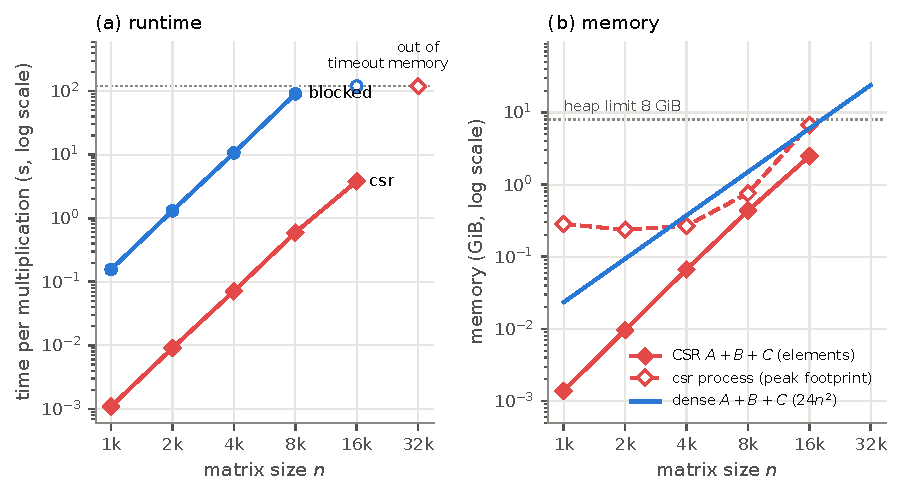
\includegraphics[width=\linewidth]{fig_size.pdf}
\caption{Part B at 1\% density (uniform). (a) Median time per multiplication;
hollow markers are the blocked timeout at $n=16384$ and the csr memory failure
at $n=32768$, drawn at the time budget. (b) Element storage of csr's
matrices, peak footprint of the csr process, and element storage of three
dense matrices.}
\label{fig:size}
\end{figure}

\subsection{The baseline in a second session}

The basic kernel and its inputs are those of Assignment~1, so its times can be
compared across the two sessions. Up to $n=512$ they agreed within 1\%. From
$n=768$ to 2048, this session was 4 to 13\% faster (for example 0.850\,s
against 0.954\,s at $n=1024$). The two sessions differ in the pre-warm, the heap
limit (8 against 4\,GiB) and the background load, so the cause cannot be
isolated.

% ===========================================================================
\section{Discussion}
\label{sec:discussion}

\paragraph{Answer to Part A.} On this machine, the loop order was the
optimisation that mattered. Reordering the baseline's loops made it 3 to 10
times faster, and the gain grew with $n$. Cache blocking, added on top, helped
only once the matrices were large, by factors of 1.2 to 1.6 at $n=3072$ and
4096, and cost up to 14\% between $n=768$ and 2048. Neither optimisation
changed the memory use.

\paragraph{HA1: loop reordering.} Supported. The counters separate two effects.
First, ikj executes far fewer instructions: 2.9 to 4.6 per multiply-add against
about 12 for basic. A scalar i-k-j iteration needs at least five instructions (two
loads, a multiply, an add and a store), so fewer than five per multiply-add
means that each instruction handled more than one element. This is consistent
with the vectorised code expected from SuperWord, 2 doubles per 128-bit
instruction~\cite{larsen2000}. The JIT output itself was not inspected. Second, ikj does not stall: its
cycles per multiply-add stayed between 0.49 and 0.63 up to $n=2048$, while
basic's rose from 1.5 to 9.3 for the same instructions. This is the effect that Assignment~1
attributed to the column walk over $B$. The row-wise access of ikj removes it
until $n=2048$. The growing gap between the two methods is therefore the
baseline's stall cycles, and the constant factor of about 3 at small $n$ is the
instruction count.

\paragraph{HA2: cache blocking.} Partly supported. As predicted, blocking
gained nothing while ikj ran without stalls, and L1-sized tiles were the worst
choice: at $n=2048$, tiles of 32 made the kernel 1.47 times slower than ikj. The
blocked loop executes the same inner loop as ikj with a shorter trip count
($b$ instead of $n$) and more loop control, which shows as 0.2 to 0.5 more
instructions per multiply-add from $n=768$ upward. Blocking paid off exactly where ikj's cycles per
multiply-add rose, at $n=3072$ (0.96) and 4096 (0.79), while blocked stayed at
0.62. At those sizes $B$ takes 72 and 128\,MiB and is read in full once per row
of $A$, whereas blocked rereads a 2\,MiB tile of $B$ from the L2 cache. The
prediction was wrong in one detail: ikj ran slower per multiply-add at
$n=3072$ than at 4096. Without cache and TLB miss counters this cannot be
explained, and it is the largest anomaly of Part~A.

\paragraph{HA3 and HA4: results and memory.} Supported. All methods agreed bit
for bit in every check and in every benchmark checksum, which confirms that
they perform the same operations in the same order. The peak RSS of the three
dense methods differed by at most 1.1\,MiB, so the optimisations changed
runtime only. Above the baseline, RSS exceeded the element storage by 28 to
58\% at the largest sizes. This is plausibly the G1 heap growing in large steps,
as in Assignment~1, but heap use was not recorded.

\paragraph{Answer to Part B.} The CSR product was faster than the optimised
dense method by factors of 7 to 26\,000 at every tested density up to 10\%, and
2.6 times slower at 50\%. Its advantage depended on the structure, on whether
the inputs had to be converted, and on how much the product filled in, not on
the density alone.

\paragraph{HB1: what the sparse kernel costs.} Partly supported. The dense
time was independent of the density (within 2.3\%), as predicted, because the
dense kernels perform all $n^3$ multiply-adds whatever the values. The sparse
time did not simply follow the multiply-add count. Its cost per multiply-add
fell from 15\,ns to 1.6\,ns as the density rose. At low densities, each
multiply-add creates a new entry of $C$ (209\,817 entries for 215\,197
multiply-adds at 0.5\%, uniform). Each entry must be marked in both passes,
written, and ordered within its row. At 0.5\% the rows of $C$ hold about 100
entries and are sorted, which by itself is on the order of a million
comparisons. At high densities, most multiply-adds hit an entry that already
exists, and the cost approaches that of the accumulation loop alone. The
phases were not timed separately, so this breakdown is an explanation
consistent with the counts, not a measurement.

\paragraph{HB2: structure, not density alone.} Supported. Uniform and banded
inputs had the same density, the same nonzero count and the same multiply-add
count within 1.6\% (up to 10\%). Yet the banded products had 2.8 to 5.3 times
fewer nonzeros, and csr ran 1.2 to 2.2 times faster on them. The difference
comes from the output: in a banded product, the contributions to a row of $C$
overlap in a narrow band of columns, so many multiply-adds fall on existing
entries and the accumulator is accessed in a small window. At 50\% the band
covers three quarters of the matrix and both products are full, so the
structures behaved the same. A percentage of zeros alone therefore did not
determine the cost in these experiments.

\paragraph{HB3: break-even with the dense method.} Partly supported. csr won up
to 10\% and lost at 50\% for both structures, as predicted. The banded inputs
gave a larger advantage at every density up to 10\%, but the interpolated
break-even was about the same, near 30\%, for both structures. Between 10 and
50\% the band widens until the two structures converge. Densities between 10
and 50\% would be needed to locate the break-even.

\paragraph{HB4 and HB5: storage and conversion.} Supported. CSR stored the
inputs in less space than the dense form at every tested density (48 against
64\,MiB at 50\%). For uniform inputs from 5\% upward, the product filled in, and
its CSR form became 1.5 times the size of a dense $C$. When the inputs arrive in
dense form, converting them costs $O(n^2)$, 7.4\,ms at $n=2048$, and at 0.1\%
density this conversion was 127 times the product itself. It cut the speed-up
from about 22\,000 to 152. The conversion back to dense was cheaper, and from
5\% upward both conversions were small next to the product. Whether sparse
storage pays off at very low densities therefore depends on whether the data
already exists in a sparse format.

\paragraph{HB6: the largest feasible size.} Supported. At 1\% density, csr kept an
advantage of about 150 times up to $n=8192$, and both methods grew roughly as $n^3$,
because the multiply-add count $n^3d^2$ is cubic for a fixed density. The dense
method stopped at the time budget at $n=16384$. The sparse one stopped at the
heap limit at $n=32768$, because the density of $C$ approached 100\%. Its product
would have needed about 12.4\,GB, more than the dense form of $C$ (8.6\,GB).
The multiply-adds alone ($3.5\times10^9$) would have fitted the time budget:
at the 9 to 11\,ns per multiply-add measured at 1\% density, they need about
30 to 40\,s. At a fixed density, the output, not the
arithmetic, limits the sparse product. The process footprint at $n=16384$ (6.7\,GiB
against 2.5\,GiB of element storage) also shows that a garbage-collected
runtime needs headroom: the previous product stays in the heap until it is
collected.

\paragraph{Optimisation versus storage.} The two parts measure different
effects and should not be merged. The dense optimisations changed the cost of
the same $n^3$ multiply-adds, by factors of 3 to 15. Sparse storage changed
the work itself: at $n=2048$ it reduced the multiply-adds by factors of 4 (50\%
density) to 1\,000\,000 (0.1\%), and the structure then set the size of the
output. The comparator also
matters for the conclusion. Against the baseline (12.2\,s at $n=2048$) instead
of blocked, the csr product would be about 3.6 times \emph{faster} at 50\%
density. That figure is derived from the baseline's time on the dense inputs,
since dense time does not depend on the density, and it was not measured on the
sparse inputs. An unoptimised dense comparator would move the break-even above
50\%. Every sparse speed-up in this report is therefore relative to the
optimised dense method.

\paragraph{Limitations.}
\begin{itemize}
  \item \textbf{One machine, one session.} Each configuration has five samples
  from one session on a fanless laptop with desktop applications open (load
  average 5.1 at the start, 2.0 at the end). The IQRs describe variability
  within the session. The baseline's 4 to 13\% difference from Assignment~1 at
  mid sizes shows that between-session differences can exceed them.
  \item \textbf{No miss counters, no JIT output.} Cache and TLB misses were not
  measured, and the JIT-compiled code was not disassembled. Vectorisation is
  inferred from instruction counts. The causes proposed for the blocking gain
  and for ikj's anomaly at $n=3072$ are inferences.
  \item \textbf{Sparse phases.} The symbolic pass, the numeric pass and the
  ordering of columns were timed together, so their shares are inferred.
  \item \textbf{Synthetic inputs.} Only two structures were tested, both with
  nearly equal row lengths. Real sparse matrices (graphs with skewed degrees,
  meshes) may behave differently. Densities between 10 and 50\% were not tested.
  \item \textbf{Memory metrics.} Peak RSS and footprint cover the whole JVM,
  including garbage, and at $n=2048$ they hide the differences in element
  storage. Element storage ignores object headers and csr's work arrays
  ($12n$ bytes).
  \item \textbf{Pilot-chosen tile size.} The tile size of 512 was chosen from a
  pilot on the same machine, so it favours blocked on this machine.
  Experiment A\_block shows how much the choice matters.
  \item \textbf{Pre-warm.} The pre-warm compiles each method on small inputs.
  It removed the OSR/C1 effect observed in the pilot, and the first full-size
  warm-up samples matched the measured ones. A long-running application could
  still reach a different compiled state.
\end{itemize}

% ===========================================================================
\section{Conclusions}
\label{sec:conclusions}

For the tested methods, inputs and machine, this study establishes the
following:
\begin{enumerate}
  \item All methods, dense and sparse, produce bitwise-identical results,
  because each adds the products of every $C_{ij}$ in increasing $k$ without
  fused multiply-add.
  \item Reordering the loops to i-k-j makes the Java kernel 3 to 10 times faster
  than the i-j-k baseline. It cuts the instructions per multiply-add by a factor
  of 2.7 to 3.9, a count consistent with vectorised code, and removes the baseline's
  stall cycles up to $n=2048$.
  \item Cache blocking on top of i-k-j does not help while the i-k-j stream
  through $B$ runs without stalls ($n\le2048$), where it costs up to 14\%. It
  gains 1.2 to 1.6 times at $n=3072$ and 4096. L2-sized tiles beat L1-sized
  ones. Neither optimisation changes the memory use.
  \item The CSR product beats the blocked dense method by factors of 7 to
  26\,000 at densities from 0.1 to 10\%, and loses by a factor of 2.6 at 50\%
  ($n=2048$).
  \item Density alone does not determine the sparse cost. At equal density and
  equal multiply-adds, banded inputs fill in up to 5.3 times less and run up to
  2.2 times faster than uniform ones.
  \item Converting dense inputs to CSR outweighs the sparse product below about
  1\% density at $n=2048$. The fill-in of the product makes its CSR form larger
  than the dense form for uniform inputs from 5\% density.
  \item At a fixed density of 1\%, the dense method reaches $n=8192$ within the
  120\,s budget and the sparse one reaches $n=16384$; the sparse product then
  fails on the memory of its output, not on time.
\end{enumerate}
Three questions remain open. The first is why i-k-j runs slower per
multiply-add at $n=3072$ than at 4096. The second is where the break-even
density lies between 10 and 50\%. The third is how much each phase of the
sparse product (symbolic pass, accumulation, ordering of the output) contributes.
Cache and TLB miss counters, a finer density grid and phase timers would answer
them.

% ===========================================================================
\section{References and materials}
\label{sec:materials}

\paragraph{Reproducibility materials.} All code, data and scripts are in the
directory \texttt{assignment2/} of the GitHub repository below, at the tag
\texttt{assignment2-v1.0}:
\begin{center}\repourl\end{center}
Its README gives the exact build and run commands and the software versions.
The materials are:
\begin{itemize}
  \item \texttt{src/}: the Java methods, the benchmark driver and the JUnit tests;
  \texttt{pom.xml}: the Maven build.
  \item \texttt{config/bench.json}: the declared protocol, read by every script.
  \item \texttt{scripts/}: input generation (\texttt{gen\_inputs.py}),
  correctness verification (\texttt{verify.py}), the benchmark harness
  (\texttt{run\_benchmarks.py}) and the environment snapshot.
  \item \texttt{data/checksums.sha256}: the digests of the inputs, which are
  regenerated in a few seconds instead of being stored.
  \item \texttt{results/correctness.csv}: the outcome of the correctness checks.
  \item \texttt{results/raw/\session/}: every raw sample, warm-ups included
  (\texttt{samples.csv}), one row per process with status, nonzero counts, peak
  RSS and counters (\texttt{runs.csv}), the environment snapshot
  (\texttt{env.txt}) and the protocol used (\texttt{config.json}).
  \item \texttt{analysis/analyze.py}: the script that produces every table and
  figure in this report from the raw data.
\end{itemize}

\paragraph{Reuse of Assignment 1.} The baseline kernel, the dense input
generator and the dense input files, the correctness tolerance, and the
structure of the benchmark harness, the verification script and the analysis
script come from Assignment~1 at the tag \texttt{assignment1-v1.0}. The reused
files are adapted copies, and each one names its origin.

\paragraph{Use of generative AI.} Claude Code (Anthropic, model Claude Opus~5.5)
was used as a programming and writing assistant. It helped plan the study, draft
and debug the Java code, tests, scripts and analysis, diagnose the JIT warm-up
problem found in the pilot, and draft and revise the text of this report. All
measurements were produced by running the code on the author's machine, and
every result in Section~\ref{sec:results} is computed from the committed data by
the scripts in the repository. Each cited source was checked against the
original publication or documentation. The author reviewed the code and the
text and is responsible for the work and its conclusions.

\renewcommand{\refname}{References}
\begin{thebibliography}{99}\raggedright
\small

\bibitem{bryant2016}
R.~E. Bryant and D.~R. O'Hallaron, \emph{Computer Systems: A Programmer's
Perspective}, 3rd~ed. Boston, MA, USA: Pearson, 2016, ch.~6.

\bibitem{drepper2007}
U.~Drepper, ``What every programmer should know about memory,'' Red Hat, Inc.,
Nov. 2007. [Online]. Available: \url{https://www.akkadia.org/drepper/cpumemory.pdf}

\bibitem{larsen2000}
S.~Larsen and S.~Amarasinghe, ``Exploiting superword level parallelism with
multimedia instruction sets,'' in \emph{Proc. ACM SIGPLAN Conf. Programming
Language Design and Implementation (PLDI)}, 2000, pp.~145--156,
doi: 10.1145/349299.349320.

\bibitem{lam1991}
M.~D. Lam, E.~E. Rothberg, and M.~E. Wolf, ``The cache performance and
optimizations of blocked algorithms,'' in \emph{Proc. 4th Int. Conf.
Architectural Support for Programming Languages and Operating Systems
(ASPLOS)}, 1991, pp.~63--74, doi: 10.1145/106972.106981.

\bibitem{goto2008}
K.~Goto and R.~A. van~de Geijn, ``Anatomy of high-performance matrix
multiplication,'' \emph{ACM Trans. Math. Softw.}, vol.~34, no.~3, Art.~no.~12,
May 2008, doi: 10.1145/1356052.1356053.

\bibitem{higham2002}
N.~J. Higham, \emph{Accuracy and Stability of Numerical Algorithms}, 2nd~ed.
Philadelphia, PA, USA: SIAM, 2002.

\bibitem{jep306}
J.~Darcy, ``JEP 306: Restore always-strict floating-point semantics,''
OpenJDK, delivered in JDK~17. Accessed: Oct.~29, 2026. [Online]. Available:
\url{https://openjdk.org/jeps/306}

\bibitem{saad2003}
Y.~Saad, \emph{Iterative Methods for Sparse Linear Systems}, 2nd~ed.
Philadelphia, PA, USA: SIAM, 2003, ch.~3.

\bibitem{gustavson1978}
F.~G. Gustavson, ``Two fast algorithms for sparse matrices: Multiplication and
permuted transposition,'' \emph{ACM Trans. Math. Softw.}, vol.~4, no.~3,
pp.~250--269, Sep. 1978, doi: 10.1145/355791.355796.

\bibitem{gilbert1992}
J.~R. Gilbert, C.~Moler, and R.~Schreiber, ``Sparse matrices in MATLAB: Design
and implementation,'' \emph{SIAM J. Matrix Anal. Appl.}, vol.~13, no.~1,
pp.~333--356, 1992, doi: 10.1137/0613024.

\bibitem{davis2006}
T.~A. Davis, \emph{Direct Methods for Sparse Linear Systems}. Philadelphia, PA,
USA: SIAM, 2006, ch.~2.

\bibitem{georges2007}
A.~Georges, D.~Buytaert, and L.~Eeckhout, ``Statistically rigorous Java
performance evaluation,'' in \emph{Proc. 22nd Annu. ACM SIGPLAN Conf.
Object-Oriented Programming Systems, Languages and Applications (OOPSLA)},
2007, pp.~57--76, doi: 10.1145/1297027.1297033.

\bibitem{harris2020}
C.~R. Harris \emph{et al.}, ``Array programming with NumPy,'' \emph{Nature},
vol.~585, no.~7825, pp.~357--362, Sep. 2020, doi: 10.1038/s41586-020-2649-2.

\bibitem{virtanen2020}
P.~Virtanen \emph{et al.}, ``SciPy 1.0: Fundamental algorithms for scientific
computing in Python,'' \emph{Nature Methods}, vol.~17, no.~3, pp.~261--272,
Mar. 2020, doi: 10.1038/s41592-019-0686-2.

\end{thebibliography}

\end{document}
